\section{ML Model Results}\label{sec:results_ML}
In this section we present the results of the ML models we have trained. We then deeply inspect the best performing model,
in order to understand its features and its performance.


% --------------- Model Selection ---------------

\subsection{Model Selection}\label{subsec:results_ML_model_selection}
As previously shown by the operative flow in Figure~\ref{fig:ML_operative_flow}, there are several phases involved in the
selection of the optimal prediction model. Given our limited resources we chose to take a greedy approach by performing
the feature selection first, and then optimizing the hyperparameters at a later time for each of the three models considered.
% MATTEO
% - Matrix plot of stepwise (which is results of algorithm 1) for each model --> to justify the chosen features
\subsubsection*{Features Selection}
To reduce the amount of time spent training the models to select the best hyperparameters, it is best to first limit the
number of features considered. The selection of the most useful features was performed using a forward stepwise selection,
following a greedy a approach that aims at maximizing the accuracy. The hyperparameters were initalized with the default
values provided by the library scikit-learn.\\
As depicted in Figure~\ref{fig:stepwise_acc_logreg}, we can see that the best accuracy with the logistic regression
model is reached after the third iteration, with little improvement with respect to the model using a single feature.
This kind of model seems to favor information about communities and centrality, while the L1 and L2 measures in some cases actually worsen its performance.
\begin{figure}[H]
	\centering
	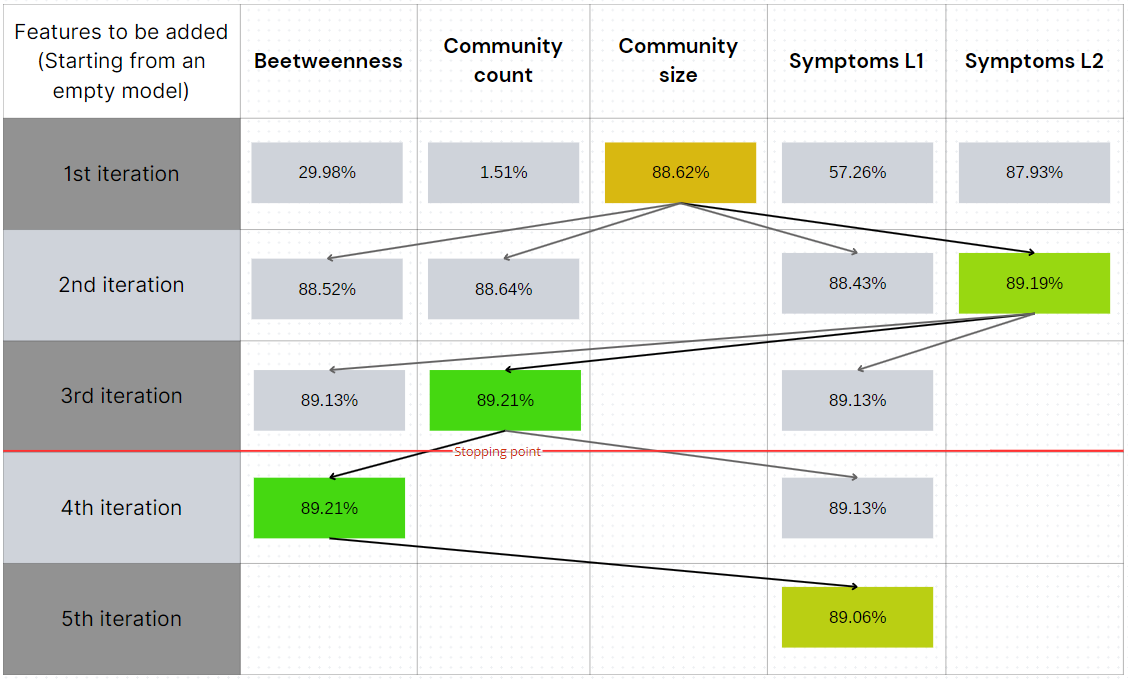
\includegraphics[width=\columnwidth]{images/stepwise_acc_logreg.png}
	\caption{Accuracy of the logistic regression models over the iterations of the forward stepwise feature selection}\label{fig:stepwise_acc_logreg}
\end{figure}
\noindent
Figure~\ref{fig:stepwise_acc_randomforest} shows that the random forest models behave similarly to the logistic regression,
as the best accuracy is reached after the same number of steps, employing the same features.
These results start to reveal which features are the best when it comes to classification.
It is also worth noting that the best random forest model has a slightly worse accuracy than logistic regression,
but that might be due to the random choice of the model's parameters.

\begin{figure}[H]
	\centering
	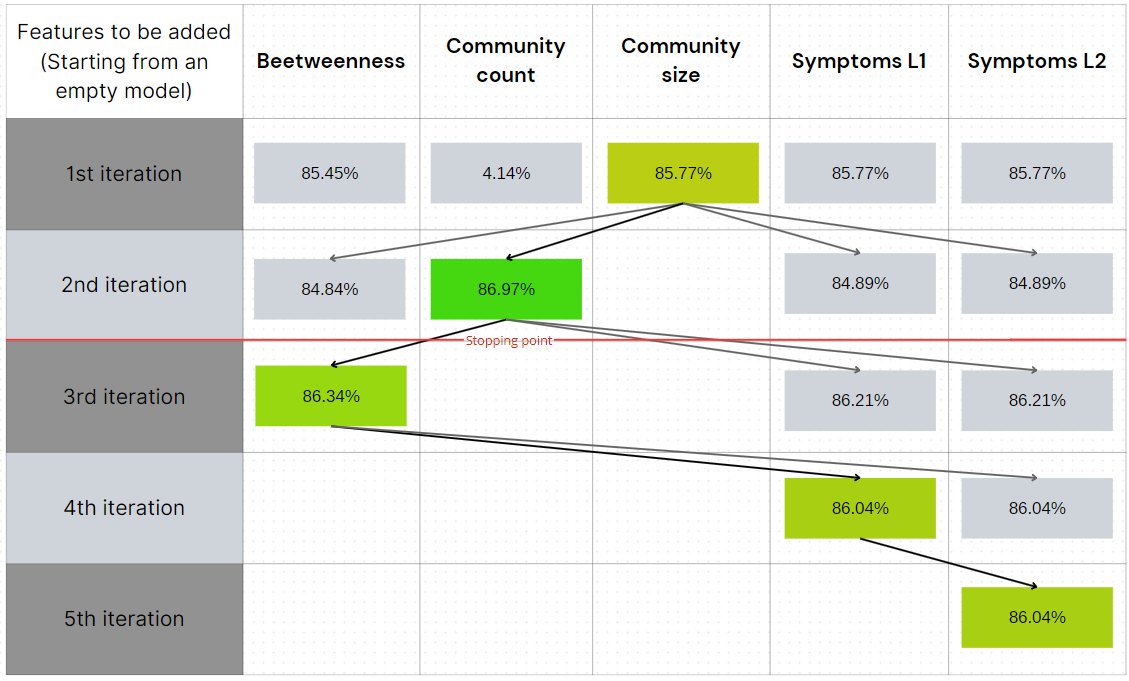
\includegraphics[width=\columnwidth]{images/stepwise_acc_randomforest.png}
	\caption{Accuracy of the random forest models over the iterations of the stepwise feature selection}\label{fig:stepwise_acc_randomforest}
\end{figure}
\noindent
The multi-layer perceptron model exhibits a different performance from the other two,
given by the fact that the accuracy starts to lower after adding the second feature.
As underlined by Figure~\ref{fig:stepwise_acc_mlp}, with respect to the other models information about the betweenness
is not needed to achieve the best possible results, which could be explained by the better ability of the MLP to adapt to non-linearities.
This particular implementation of neural network has one hidden layer with 100 neurons, and in our case its performance is better
than the random forest model, but still slightly worse than the logistic regression. We expect this to change after the optimization of the hyperparameters.

\begin{figure}[H]
	\centering
	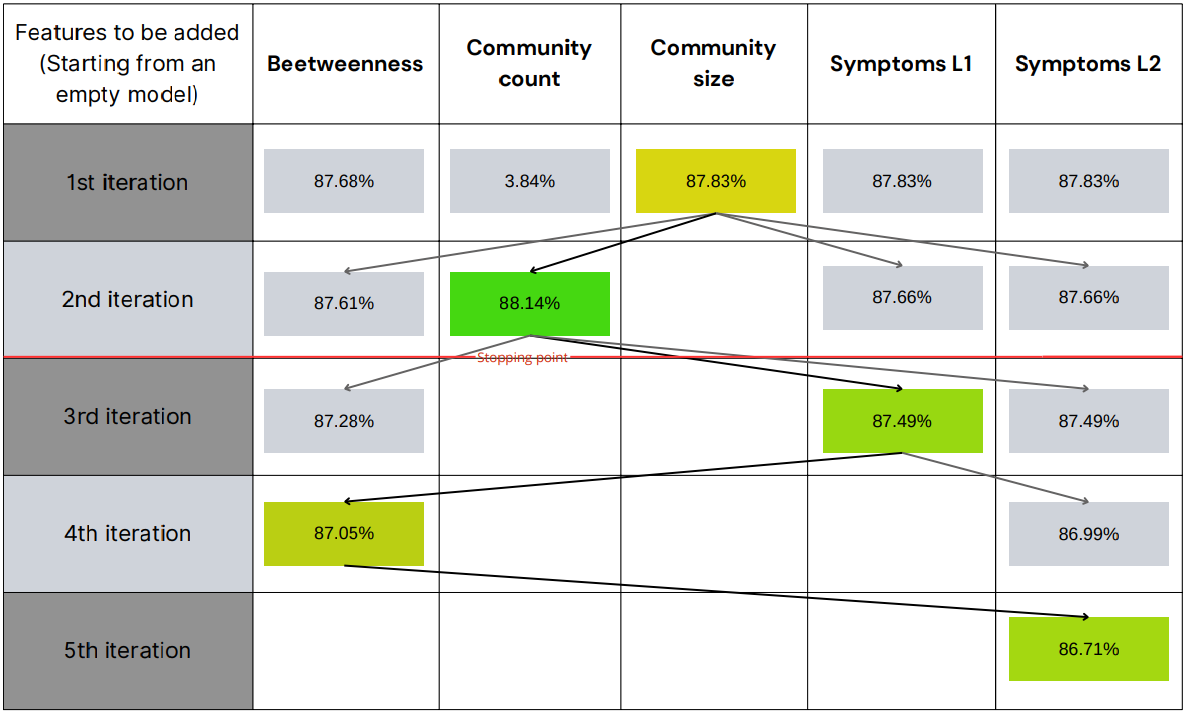
\includegraphics[width=\columnwidth]{images/stepwise_acc_mlp.png}
	\caption{Accuracy of the MLP models over the iterations of the stepwise feature selection}\label{fig:stepwise_acc_mlp}
\end{figure}


% CRISTIAN
% - Comparison for each model of the selected parameters --> to justify the chosen parameters
\subsubsection*{Hyperparameters Selection}


% ANDREA
% - Comparison of the three models with best combination of features and best parameters
% - precision, recall, AUC, accuracy
\subsubsection*{Model Comparison}\label{subsubsec:results_ML_model_comparison}

As illustrated in Figure~\ref{fig:ML_operative_flow}, our model ensemble now comprises six variants:
three leveraging only symptoms and three incorporating new network-based features. The selection of
the best-performing model from each group was based on test accuracy assessment, where the test is the same balanced dataset
in all cases. Figure~\ref{fig:acc_symptoms}
illustrates consistently low overfitting across all models, showcasing the stability of the symptom-only
models. In contrast, Figure~\ref{fig:acc_new_features}, portraying the accuracy of models with the new
features, reveals some overfitting, particularly in the MLP and Random Forest.\\
The observed tendency for models with new features to exhibit more pronounced overfitting is unsurprising,
given the greater number and complexity of these features compared to symptoms. Notably, despite their different
complexity, all models demonstrate similar test accuracy levels, suggesting that a linear separation
boundary suffices for effective feature classification. Considering this, we retain the Logistic Regression
model as the best-performing model in each group, striking a balance between performance and complexity.

\begin{figure}[H]
	\centering
	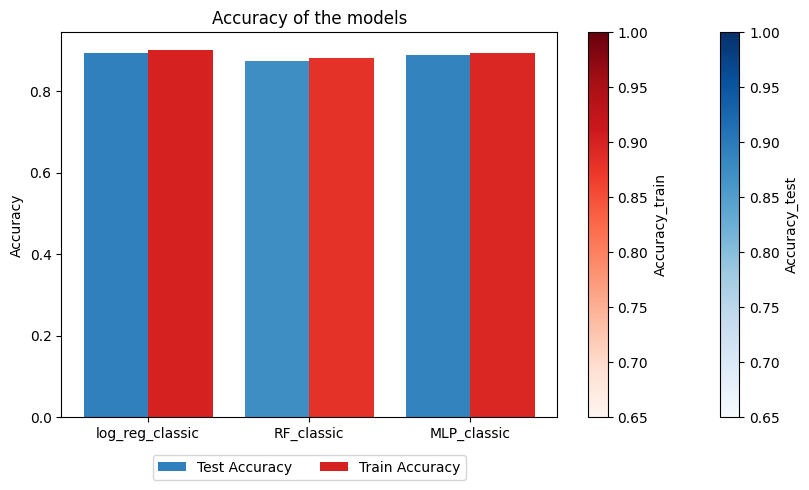
\includegraphics[width=\columnwidth]{images/acc_symptoms.png}
	\caption{Accuracy of the three models with only symptoms}\label{fig:acc_symptoms}
\end{figure}

\begin{figure}[H]
	\centering
	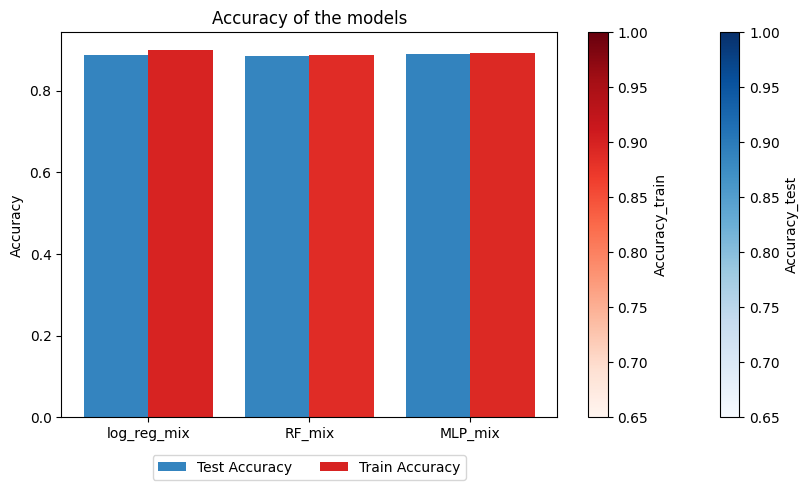
\includegraphics[width=\columnwidth]{images/acc_new_features.png}
	\caption{Accuracy of the three models with new features}\label{fig:acc_new_features}
\end{figure}



% --------------- New Features Effect ---------------

\subsection{New Features Effect}
% ANDREA
% - compare the best symptoms one hot model with the best one with the new features

\noindent
The best model from each group was further trained on the full balanced dataset to ensure a more reliable
performance evaluation. The results in Figure~\ref{fig:acc_best_models} reveal a minimal difference between
the two groups. This addresses our \textbf{first goal}: the new features, while not improving the model,
offer a comparable performance to using symptoms alone. However, It's essential to note that the new features are
more numerous than the symptoms, contributing to a more complex model. In conclusion, the extracted network
features are not a superior alternative to symptoms.

It is worth to underline that the `simplicity' of the dataset, which leads to a very high accuracy in all models, may also affect the performance
evaluation of the new features, which have a small room to improve the model. Therefore, a possible avenue
for future exploration could involve the use of more complex dataset, to better assess the performance of the
new features.

Another viable option for future work is to use the new features as a complement to the symptoms.


% THE FIGURE IS THE FIGURE OF MODEL FULLY TRAINED ON THE BALANCED DATASET


\begin{figure}[H]
	\centering
	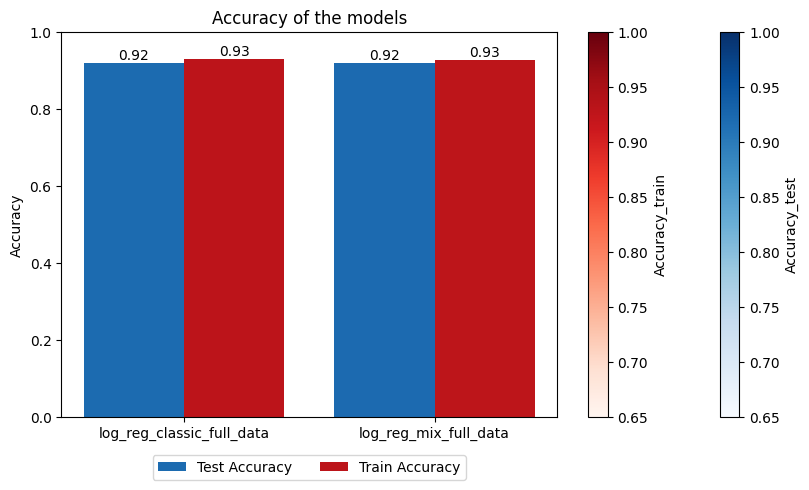
\includegraphics[width=\columnwidth]{images/acc_best_models.png}
	\caption{Accuracy of the best models from both groups}\label{fig:acc_best_models}
\end{figure}



% --------------- Best Model Performance ---------------

\subsection{Best Model Analysis}
% DAVIDE
% - what are its features
% - confusion matrix computed on the 4 class diseases (HighL1 - HighL2, LowL1 - HighL2, ...)
% - Worst error
% - Most impactful symptoms



\subsection{Computational Complexity}
% MATTEO
% - apply the reduction technique based on symptoms importance (L1 and L2 combined in the 4 classes)
% - compare the performance of the reduced model with the original one
% - precision, recall, AUC, accuracy
% - compare the times needed to train the two models


% CRISTIAN
% - 6 Modelli: 3 con solo sintomi, 3 con nuove features
% - - Salvati (joblib) 
% - - Tempo di training

